% \documentclass{beamer}

% \usepackage[brazil]{babel}
% \usepackage[utf8x]{inputenc}

% \title{Método Automático de Contagem Volumétrica de Veículos baseado em Visão Computacional}
% \author{Arthur Ferreira Bailão}

% \begin{document}
%   \frame{\titlepage}

%   \section{Sumário}
%   \frame{\tableofcontents}
  
% \end{document}

% $Header: /Users/joseph/Documents/LaTeX/beamer/solutions/conference-talks/conference-ornate-20min.en.tex,v 90e850259b8b 2007/01/28 20:48:30 tantau $

\documentclass{beamer}

% This file is a solution template for:

% - Talk at a conference/colloquium.
% - Talk length is about 20min.
% - Style is ornate.



% Copyright 2004 by Till Tantau <tantau@users.sourceforge.net>.
%
% In principle, this file can be redistributed and/or modified under
% the terms of the GNU Public License, version 2.
%
% However, this file is supposed to be a template to be modified
% for your own needs. For this reason, if you use this file as a
% template and not specifically distribute it as part of a another
% package/program, I grant the extra permission to freely copy and
% modify this file as you see fit and even to delete this copyright
% notice. 


\mode<presentation>
{
  \usetheme{Warsaw}
  % or ...

  \setbeamercovered{transparent}
  % or whatever (possibly just delete it)
}


\usepackage[brazil]{babel}
% or whatever

\usepackage[utf8x]{inputenc}
% or whatever
\usepackage{dcolumn}
\usepackage{times}
\usepackage{multirow}
% \usepackage[T1]{fontenc}

% Or whatever. Note that the encoding and the font should match. If T1
% does not look nice, try deleting the line with the fontenc.


\title[Contagem Volumétrica e Visão Computacional] % (optional, use only with long paper titles)
{Método Automático de Contagem Volumétrica de Veículos baseado em Visão Computacional}

% \subtitle
% {Include Only If Paper Has a Subtitle}

\author[Arthur Bailão] % (optional, use only with lots of authors)
{Arthur Ferreira Bailão{\texorpdfstring{\\\footnotesize Orientador: Prof. Hermes Aguiar Magalhães\\Supervisora: Profª. Leise Kelli de Oliveira}{\footnotesize Orientador: Prof. Hermes Aguiar Magalhães Supervisora: Profª. Leise Kelli de Oliveira}}}
% - Give the names in the same order as the appear in the paper.
% - Use the \inst{?} command only if the authors have different
%   affiliation.

\institute % (optional, but mostly needed)
{Universidade Federal de Minas Gerais}
% - Use the \inst command only if there are several affiliations.
% - Keep it simple, no one is interested in your street address.

\date % (optional, should be abbreviation of conference name)
{Projeto Final de Curso}
% - Either use conference name or its abbreviation.
% - Not really informative to the audience, more for people (including
%   yourself) who are reading the slides online

% \subject{Theoretical Computer Science}
% This is only inserted into the PDF information catalog. Can be left
% out. 



% If you have a file called "university-logo-filename.xxx", where xxx
% is a graphic format that can be processed by latex or pdflatex,
% resp., then you can add a logo as follows:

\pgfdeclareimage[height=0.5cm]{university-logo}{imgs/principal_ufmg}
\logo{\pgfuseimage{university-logo}}



% Delete this, if you do not want the table of contents to pop up at
% the beginning of each subsection:
% \AtBeginSubsection[]
% {
%   \begin{frame}<beamer>{Sumário}
%     \tableofcontents[currentsection,currentsubsection]
%   \end{frame}
% }
\AtBeginSection[]
{
  \begin{frame}<beamer>{Sumário}
    \tableofcontents[currentsection]
  \end{frame}
}

% If you wish to uncover everything in a step-wise fashion, uncomment
% the following command: 

% \beamerdefaultoverlayspecification{<+->}


\begin{document}

\begin{frame}
  \titlepage
\end{frame}

\begin{frame}{Sumário}
  \tableofcontents
  % You might wish to add the option [pausesections]
\end{frame}


% Structuring a talk is a difficult task and the following structure
% may not be suitable. Here are some rules that apply for this
% solution: 

% - Exactly two or three sections (other than the summary).
% - At *most* three subsections per section.
% - Talk about 30s to 2min per frame. So there should be between about
%   15 and 30 frames, all told.

% - A conference audience is likely to know very little of what you
%   are going to talk about. So *simplify*!
% - In a 20min talk, getting the main ideas across is hard
%   enough. Leave out details, even if it means being less precise than
%   you think necessary.
% - If you omit details that are vital to the proof/implementation,
%   just say so once. Everybody will be happy with that.

\section{Introdução} % (fold)
\label{sec:introdu_o}

\begin{frame}{O tráfego de veículos}
  Representa um fenômeno de grande importância socioeconômica. Deslocamentos no menor tempo possível, são uma necessidade cotidiana. Projetar sistemas viários exige ferramentas cujo desenvolvimento ainda representa objeto de estudo para diversos grupos de pesquisadores.
\end{frame}

\begin{frame}{A contagem volumétrica}
  Consiste em quantificar o volume de veículos trafegando em uma via, durante um intervalo de tempo. Seus resultados são subsídios básicos para estudos econômicos, projetos rodoviários e planejamento de tráfego.
  
\end{frame}

\begin{frame}{A contagem volumétrica}{Finalidades}
  \begin{itemize}
    \item Planejar o sistema rodoviário.
    \item Programar necessidades e prioridades de melhorias no sistema rodoviário.
    \item Avaliar o fluxo existente de tráfego em relação ao sistema rodoviário atual.
    \item Justificar e planejar o policiamento.
    \item Estudos de localização de postos de pesagem, socorro médico emergencial, etc.
  \end{itemize}
\end{frame}

% section introdu_o (end)

\section{Objetivos} % (fold)
\label{sec:objetivos}

\begin{frame}{O objetivo do trabalho}
  Desenvolver um método de contagem volumétrica que auxilie na análise das condições do tráfego urbano.
  \pause
  \begin{itemize}
    \item Contagem volumétrica utilizando um método não-invasivo de \alert{SIMPLES} implementação.
    \item Utilizar imagens coletadas por uma câmera digital.
    \item Determinar a qualidade do método.
    \item Identificar pontos de acerto e erro que podem ser trabalhados.
  \end{itemize}
\end{frame}

% section objetivos (end)

\section{Metodologia} % (fold)
\label{sec:metodologia}

\subsection{Premissas} % (fold)
\label{sub:premissas}

\begin{frame}{Algumas premissas foram assumidas}
  \begin{enumerate}
    \item A cena possui boa iluminação, com pouca variação ao longo do tempo.
    \item Não existem oclusões parciais ou totais entre veículos.
    \item A câmera não sofre grandes vibrações ou movimentações.
  \end{enumerate} 
\end{frame}

% subsection premissas (end)

\subsection{Fluxo de processos} % (fold)
\label{sub:fluxo_de_processos}

\begin{frame}{Fluxograma global do método de contagem}
  \begin{center}
    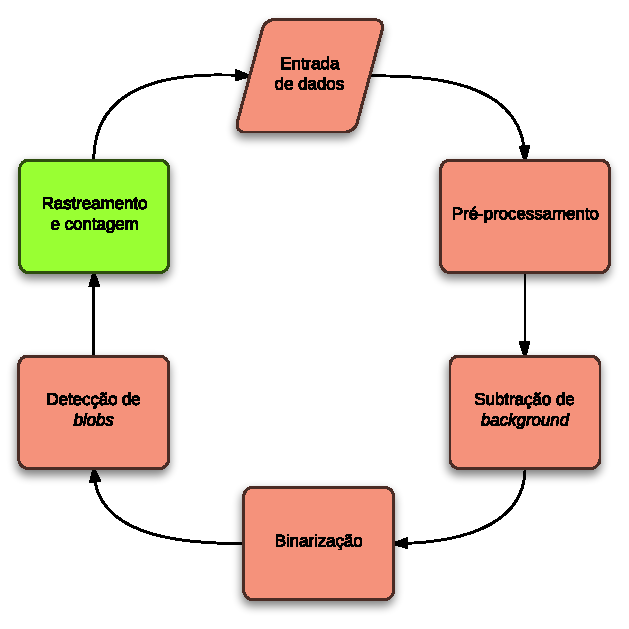
\includegraphics[scale=0.6]{imgs/general_process.pdf}
  \end{center}
\end{frame}

\begin{frame}{Entrada de dados}
  \begin{columns}[T]
    \begin{column}{.5\textwidth}
      \begin{itemize}
        \item Imagens capturadas previamente.
        \item Os \textit{frames} são obtidos individualmente.
        \item Abstração de um arquivo de vídeo por uma sequência de imagens.
      \end{itemize}
    \end{column}
    \begin{column}{.5\textwidth}
      \begin{block}{}
        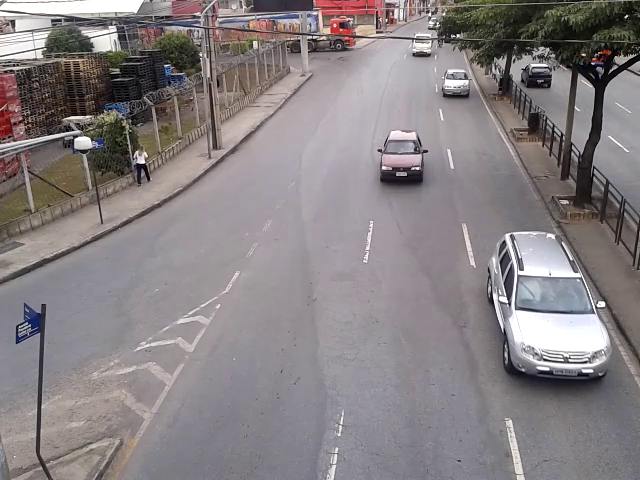
\includegraphics[width=\textwidth]{imgs/frame.png}
      \end{block}
    \end{column}
  \end{columns}
\end{frame}

\begin{frame}{Pré-processamento}
  \begin{columns}[T]
    \begin{column}{.5\textwidth}
      \begin{itemize}
        \item<1-> Conversão da imagem de entrada para \textit{grayscale}.
        \item<2-> Filtragem linear gaussiana.
      \end{itemize}
    \end{column}
    \begin{column}{.5\textwidth}
      \begin{block}{}
        \includegraphics<1>[width=\textwidth]{imgs/frame_gray.png}
        \includegraphics<2>[width=\textwidth]{imgs/gray.png}
      \end{block}
    \end{column}
  \end{columns}
\end{frame}

\begin{frame}{Subtração de \textit{background}}
  \begin{columns}[T]
    \begin{column}{.5\textwidth}
      \begin{itemize}
        \item Modelo adaptativo de mistura de gaussianas com detecção de sombras.
        \item Operação complexa e de alto custo computacional, mas de simples utilização.
      \end{itemize}
    \end{column}
    \begin{column}{.5\textwidth}
      \begin{block}{}
        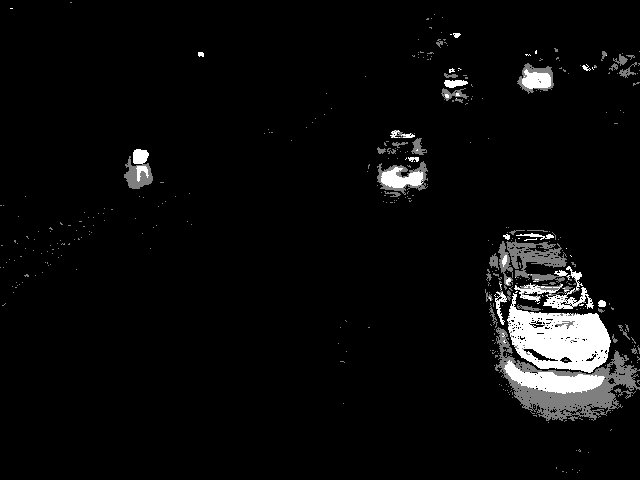
\includegraphics[width=\textwidth]{imgs/foreground.png}
      \end{block}
    \end{column}
  \end{columns}
\end{frame}

\begin{frame}{Binarização}
  \begin{columns}[T]
    \begin{column}{.5\textwidth}
      \begin{itemize}
        \item<1-> Segmentar as regiões de interesse.
        \item<1-> Operação de limiarização ou \textit{thresholding}.
        \item<2-> Operação morfológica de fechamento.
        \item<2-> Uniformizar a região de segmentação dos objetos.
      \end{itemize}
    \end{column}
    \begin{column}{.5\textwidth}
      \begin{block}{}
        \includegraphics<1>[width=\textwidth]{imgs/bin.png}
        \includegraphics<2>[width=\textwidth]{imgs/morph.png}
      \end{block}
    \end{column}
  \end{columns}
\end{frame}

\begin{frame}{Detecção de \textit{blobs}}
  \begin{columns}[T]
    \begin{column}{.5\textwidth}
      \begin{itemize}
        \item Os \textit{keypoints} definem a posição e tamanho de cada objeto segmentado.
        \item Última operação que envolve processamento de imagens.
      \end{itemize}
    \end{column}
    \begin{column}{.5\textwidth}
      \begin{block}{}
        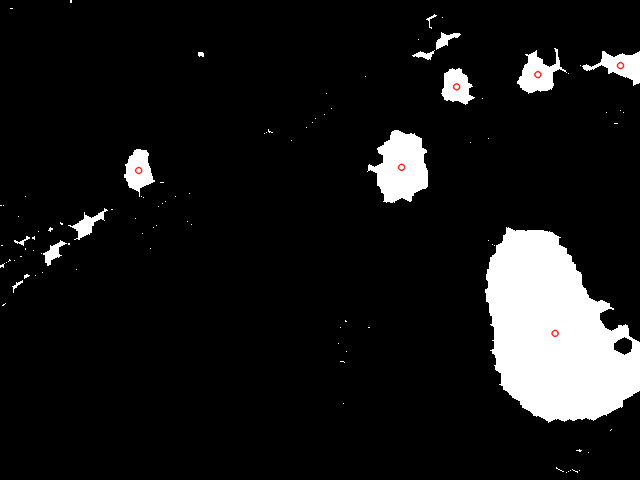
\includegraphics[width=\textwidth]{imgs/keypoints.png}
      \end{block}
    \end{column}
  \end{columns}
\end{frame}

\begin{frame}{Rastreamento e contagem}
  \begin{columns}[T]
    \begin{column}{.5\textwidth}
      \begin{itemize}
        \item Utiliza \textit{keypoints} e máscara binária.
        \item \textit{Tracker} é um objeto circular, definido por sua posição e raio.
        \item A contagem acontece se um \textit{keypoint} adentra a região de contagem e está contido por pelo menos um \textit{tracker}.
      \end{itemize}
    \end{column}
    \begin{column}{.5\textwidth}
      \begin{block}{}
        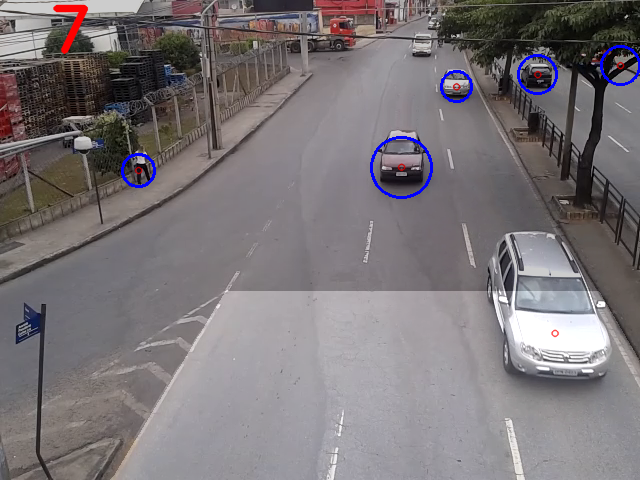
\includegraphics[width=\textwidth]{imgs/trackers.png}
      \end{block}{}
    \end{column}
  \end{columns}
\end{frame}

\begin{frame}{O algoritmo}
  \begin{center}
    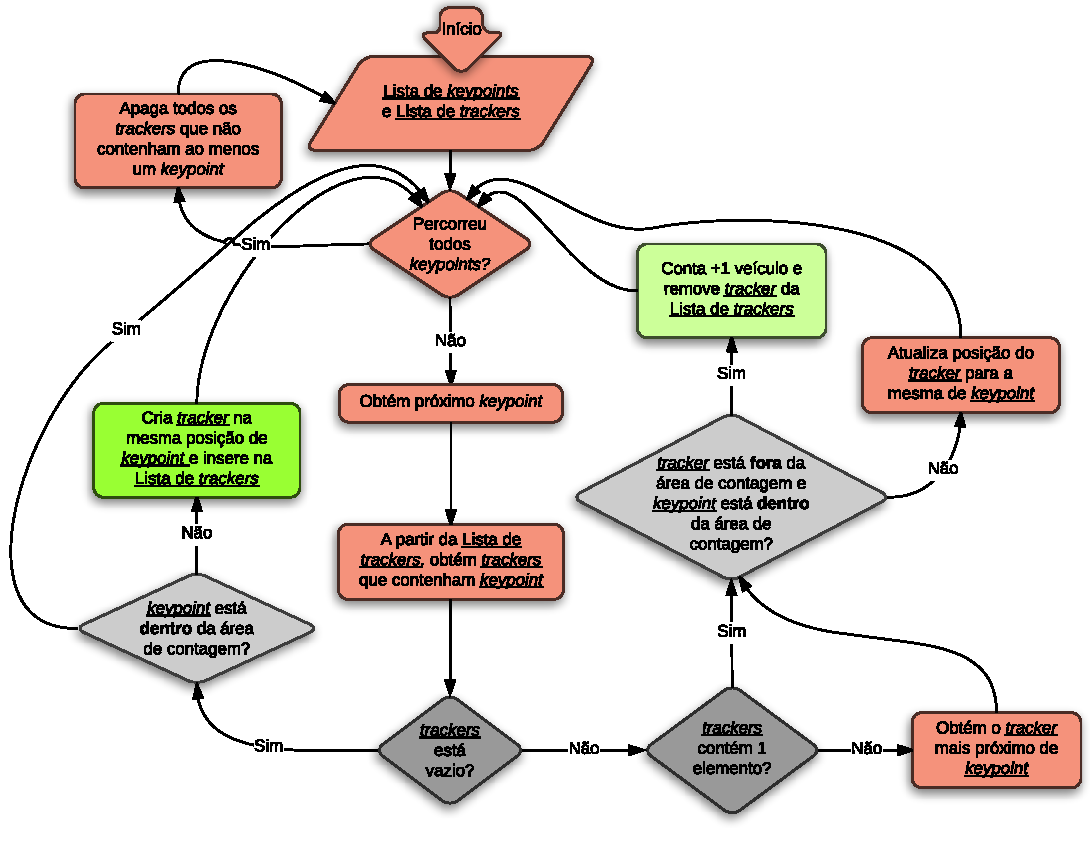
\includegraphics[scale=0.44]{imgs/fluxograma_contagem.pdf}
  \end{center}
\end{frame}

% subsection fluxo_de_processos (end)

\subsection{Avaliação dos resultados} % (fold)
\label{sub:avalia_o_dos_resultados}

\begin{frame}{A matriz de confusão}
  Contém informações sobre classificações reais e preditas feitas por um classificador.

  \begin{center}
    \begin{tabular}{l|l|c|c|}

    \multicolumn{2}{c}{} & \multicolumn{2}{c}{Classe verdadeira} \\
    \cline{3-4}
    \multicolumn{2}{c|}{} & Positivo & Negativo \\
    \cline{2-4}
    \multirow{2}{*}{Classe predita} & Positivo & VP & FP \\
    \cline{2-4}
    & Negativo & FN & VN \\
    \cline{2-4}
    
    \end{tabular}
  \end{center}
\end{frame}

\begin{frame}{Os elementos da matriz de confusão}
  \begin{itemize}
    \item Verdadeiro positivo (VP): mais um veículo foi contabilizado quando o mesmo adentrou a região de contagem em uma janela de tempo.
    \item Falso positivo (FP): mais um veículo foi contabilizado quando nenhum veículo adentrou a região de contagem em uma janela de tempo.
    \item Falso negativo (FN): mais um veículo não foi contabilizado quando o mesmo adentrou a região de contagem em uma janela de tempo.
    \pause
    \item Verdadeiro negativo (VN): mais um veículo não foi contabilizado quando nenhum veículo adentrou a região de contagem em uma janela de tempo.
\end{itemize}
\end{frame}

\begin{frame}{Os índices de desempenho}{Precisão (P), \textit{Recall} (R) e Acurácia (A)}
  \begin{equation}
    \label{eq:precisao}
    P=\dfrac{VP}{VP+FP}
  \end{equation}

  \begin{equation}
    \label{eq:recall}
    R=\dfrac{VP}{VP+FN}
  \end{equation}

  \begin{equation}
    \label{eq:acuracia}
    A=\dfrac{VP+VN}{VP+FP+FN+VN}
  \end{equation}
\end{frame}

\begin{frame}{O índice Kappa (K)}
  É utilizado como uma medida apropriada da exatidão por representar inteiramente a matriz de confusão.

  \begin{equation}
    \label{eq:kappa}
    K=\dfrac{\theta_{1}-\theta_{2}}{1-\theta_{2}}
  \end{equation}

  \begin{equation*}
    \label{eq:theta_1}
    \theta_{1}=\dfrac{VP+VN}{VP+FP+FN+VN}
  \end{equation*}

  \begin{equation*}
    \label{eq:theta_2}
    \theta_{2}=\dfrac{\alpha+\beta}{\gamma^{2}}
  \end{equation*}

  $\alpha=(VP+FN)*(VP+FP)$, $\beta=(VN+FN)*(VN+FP)$ e $\gamma=VP+VN+FP+FN$.

\end{frame} 

\begin{frame}{Determinando a qualidade da contagem}{Índice Kappa (K)}
  \begin{center}
    \begin{tabular}{cc}
    \hline
    \textbf{Índice Kappa (K)} & \textbf{Qualidade} \\
    \hline
      $K < 0.2$ & Ruim \\
      $0.2 \leq K < 0.4$ & Razoável \\
      $0.4 \leq K < 0.6$ & Bom \\
      $0.6 \leq K < 0.8$ & Muito bom \\
      $K \geq 0.8$ & Excelente \\
    \hline
    \end{tabular}
  \end{center}
\end{frame}

% subsection avalia_o_dos_resultados (end)

% section metodologia (end)

\section{Resultados} % (fold)
\label{sec:resultados}

\begin{frame}{O resultado obtido}
  \resizebox{\linewidth}{!}{
    \begin{tabular}{c|cccc|cccccc|cc}
    \textbf{Nº} & \textbf{VP} & \textbf{VN} & \textbf{FP} & \textbf{FN} & \textbf{E} & \textbf{VPN} & \textbf{P} & \textbf{R} & \textbf{FM} & \textbf{A} & \textbf{K} & \textbf{Qualidade} \\
    \hline
      1 & 92 & 35 & 2 & 6 & 0.95 & 0.85 & 0.98 & 0.94 & 0.96 & 0.94 & 0.86 & Excelente\\
      2 & 76 & 34 & 6 & 10 & 0.85 & 0.77 & 0.93 & 0.88 & 0.90 & 0.87 & 0.71 & Muito bom\\
      \hline
      3 & 107 & 19 & 1 & 26 & 0.95 & 0.42 & 0.99 & 0.80 & 0.89 & 0.82 & 0.49 & Bom \\
      4 & 87 & 28 & 8 & 22 & 0.78 & 0.56 & 0.92 & 0.80 & 0.85 & 0.79 & 0.51 & Bom \\
      5 & 94 & 37 & 2 & 15 & 0.95 & 0.71 & 0.98 & 0.86 & 0.92 & 0.89 & 0.73 & Muito bom\\
    \end{tabular}}

    \pause
    \begin{itemize}
      \item Destaque para boa precisão.
      \item Variação na qualidade entre as amostram de diferente sentido da via.
    \end{itemize}
\end{frame}

\begin{frame}{Tipo de tráfego encontrado}
  \begin{columns}[T]
    \begin{column}{.5\textwidth}
      \begin{block}{}
        \includegraphics<1>[width=\textwidth]{imgs/veiculo_grande.png}
        \includegraphics<2>[width=\textwidth]{imgs/camera_moveu.png}
      \end{block}
    \end{column}
    \begin{column}{.5\textwidth}
      \begin{itemize}
        \item Veículos de grande porte podem gerar vibração da câmera e oclusões.
        \item Movimentação da câmera causa falsas detecções.
      \end{itemize}
    \end{column}
  \end{columns}
\end{frame}

\begin{frame}{Problemas no processamento de imagens}
  \begin{columns}[T]
    \begin{column}{.5\textwidth}
      \begin{block}{}
        \includegraphics<1>[width=\textwidth]{imgs/problema_veiculo_grande.png}
        \includegraphics<2>[width=\textwidth]{imgs/problema_veiculo_junto.png}
      \end{block}
    \end{column}
    \begin{column}{.5\textwidth}
      Problemas na subtração de \textit{background} e detecção de \textit{blobs}. Possíveis melhorias:
      \begin{itemize}
        \item Pontos fiduciais para compensar a movimentação da câmera.
        \item Detectar \textit{features} para rastrear os veículos.
      \end{itemize}
    \end{column}
  \end{columns}
\end{frame}

% section resultados (end)

\section{Considerações finais} % (fold)
\label{sec:considera_es_finais}

\begin{frame}{Objetivos alcançados}
  \begin{itemize}
    \item Método proposto de simples implementação.
    \item Contagem volumétrica automática com boa precisão.
    \item Análise crítica dos resultados. 
  \end{itemize}
\end{frame}

\begin{frame}{Trabalhos futuros}
  \begin{itemize}
    \item Contagem de veículos no período noturno, em locais com baixa iluminação ou alta variação de luminosidade.
    \item Rastrear veículos utilizando \textit{features} e não \textit{blobs}.
    \item Minimizar o prejuízo causado pela movimentação da câmera pelo uso de pontos fiduciais.
    \item Criação de técnicas para classificação de veículos quanto ao tamanho.
    \item Contagem de veículos em cruzamentos, com deslocamentos em várias direções e sentidos.
    \item Estimação do volume do tráfego em vias congestionadas.
  \end{itemize}
\end{frame}

% section considera_es_finais (end)


% \section*{Summary}

% \begin{frame}{Summary}

%   % Keep the summary *very short*.
%   \begin{itemize}
%   \item
%     The \alert{first main message} of your talk in one or two lines.
%   \item
%     The \alert{second main message} of your talk in one or two lines.
%   \item
%     Perhaps a \alert{third message}, but not more than that.
%   \end{itemize}
  
%   % The following outlook is optional.
%   \vskip0pt plus.5fill
%   \begin{itemize}
%   \item
%     Outlook
%     \begin{itemize}
%     \item
%       Something you haven't solved.
%     \item
%       Something else you haven't solved.
%     \end{itemize}
%   \end{itemize}
% \end{frame}



% % All of the following is optional and typically not needed. 
% \appendix
% \section<presentation>*{\appendixname}
% \subsection<presentation>*{For Further Reading}

% \begin{frame}[allowframebreaks]
%   \frametitle<presentation>{For Further Reading}
    
%   \begin{thebibliography}{10}
    
%   \beamertemplatebookbibitems
%   % Start with overview books.

%   \bibitem{Author1990}
%     A.~Author.
%     \newblock {\em Handbook of Everything}.
%     \newblock Some Press, 1990.
 
    
%   \beamertemplatearticlebibitems
%   % Followed by interesting articles. Keep the list short. 

%   \bibitem{Someone2000}
%     S.~Someone.
%     \newblock On this and that.
%     \newblock {\em Journal of This and That}, 2(1):50--100,
%     2000.
%   \end{thebibliography}
% \end{frame}

\end{document}

